\chapter{不等价结构的生成和查重算法}\label{chapter:unique}
通过第一性原理来计算和预测材料的热力学稳定构型是计算材料学近几十年的一个重要发展。尽管这个问题很困难,但由于其重要的应用价值,该问题吸引了许多的研究关注。因为计算过程的自由度和搜索的空间十分巨大,简单的结果往往来自对大量的材料构型进行计算,同时又因为第一性原理的能量计算的计算资源耗费较大,这个问题变得十分困难。这个问题被称作晶体结构预测问题(CSP),近些年发展了非常多的方法来解决这一问题,我们在第\ref{chapter:workflows}章中已经简要介绍了相关的全局材料搜索和高通量的材料搜索方法。

这一章我们主要介绍晶体结构预测问题(CSP)的子集,即在晶格类型已知的构型中的晶格衍生结构预测的算法和实现。
这个问题虽然是原问题的子集但它同样非常重要,实验发现许多半导体或金属间形成的合金都是通过这种固定的晶格的形式形成合金。我们通过自己编写的软件实现了产生不等价的构型,并将这个方法用到了本论文的相关工作中。枚举产生的不等价的结构产生后会进一步进行结构的优化到达势能面的局域极小值点,再对比这些局域极小值点的结构的能量,以得到最稳定的构型,从而用于确定热力学稳定性的搜索过程。

\begin{figure}
  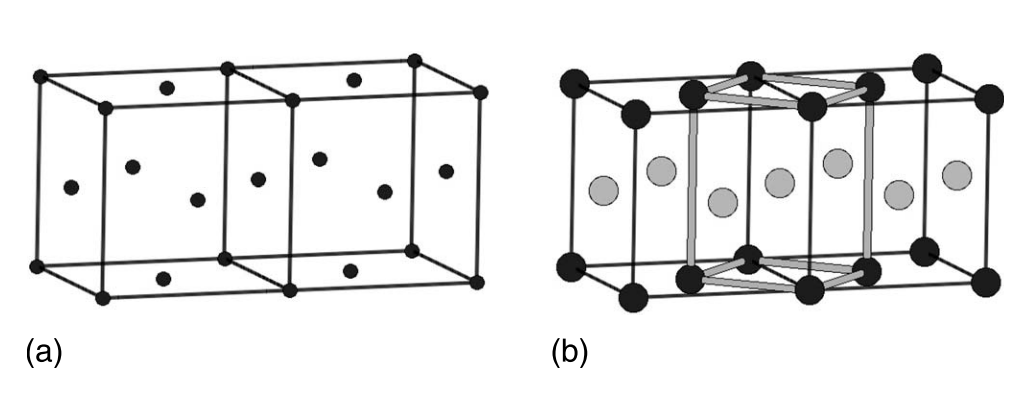
\includegraphics[width=0.72\textwidth]{figs/ch4_fcc_superlattice.png}
  \centering
  \caption{左边是原面心立方晶格,右边是原晶格扩充的超晶格,超晶格是由灰色的双单元格定义的。超晶格的两个内部点被一个黑色原子和一个灰色原子所占据。超晶格和原子一起构成了一种衍生结构。这个例子的所对应的真实合金是\ce{CuAu}合金。}
  \label{fig:ch4_fcc_superlattice}
\end{figure}

合金中的化学序结构,磁性材料中的磁序结构,以及非化学配比的带有缺陷序的材料表现出各种不同的性质都与其原超结构的衍生结构\cite{buerger1947derivative,santoro1973coincidence,santoro1972properties}有关。同样的还有超晶格的衍生结构,它是孪晶中影响结构和性质的重要因素之一。那么什么是超结构的衍生结构呢?这里我们定义其为单胞是其原单胞数倍拓展而来,原子坐标的基矢是原单胞对应的向量加和,但原子排列不同于原单胞的构型。
比如许多金属间化合物可以认为是由面心立方而来的超结构,如图\ref{fig:ch4_fcc_superlattice}所示,(b)中的构型的原子占有面心立方晶格所处的原子处,但因为其有两种原子所以不再有面心立方的对称性,而成为图\ref{fig:ch4_fcc_superlattice}(a)面心立方结构的衍生的超结构。图\ref{fig:ch4_fcc_234_ss}中展示了面心立方晶格的两倍三倍,四倍超胞的各种晶格以及所拥有的衍生超结构。

\begin{figure}
  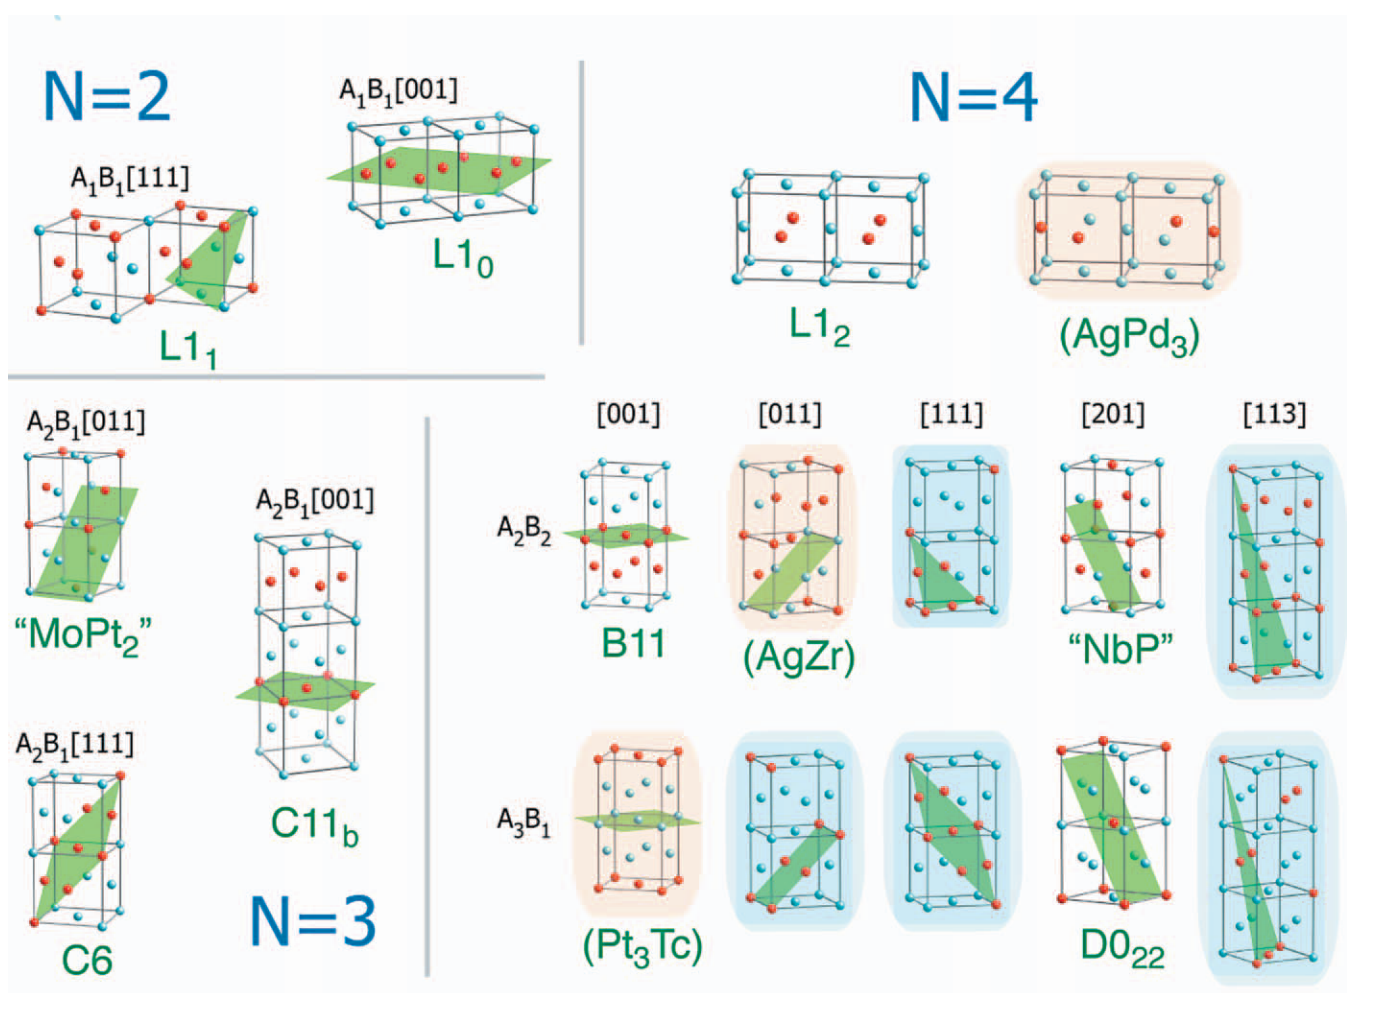
\includegraphics[width=0.96\textwidth]{figs/ch4_fcc_234_ss.png}
  \centering
  \caption{来源于面心立方晶格的前17种二元结构。超胞体积胞为原胞的二倍三倍或四倍。绿色平面所示的结构可以看作由纯A和B原子层叠加而成。例如,左上角的$L_{10}$结构是一个交替的\ce{A1B1}层序,沿001方向堆叠。所有的二倍和三倍于原晶胞的结构都有实际的物理材料的对应。在四倍的超晶格中,有4种构型具有实际的物理材料对应。其他三个黄色背景的构型已经被文献\cite{curtarolo2005accuracy}预测存在,但还没有被实验合成。另外五种蓝色背景的构型是从未被观测到或预测存在于任何系统中的。图片来源文献\cite{hart2008algorithm}}
  \label{fig:ch4_fcc_234_ss}
\end{figure}

生成的衍生结构的集合通常会被用于如确定固定晶格的二元金属间合金的基态性质。同时该方法也不仅限于搜索构型的能量,只要能够定义和有序构型有关的哈密顿量,就能描述其他的物理性质,比如Graf等\cite{graf2005direct}通过定义经验赝哈密顿量来直接预测半导体合金的带系和费米能级处电子的有效质量。只要所需要的物理性质和衍生结构构型是有关联的,就可以通过这种构建赝哈密顿量方法来建立构型和性质的联系从而搜索并预测合金的性质。

为避免重复的计算,我们需要获得衍生结构的集合(数学上的集合概念的推广,该集合中任意两个构型物理上是不等价的)。构型和构型之间的几何表示可能并不相同,但由于晶体结构的对称性,两种不同表示的结构可能会是物理上等价的,论文本章的后续章节就是描述了解决这一问题的算法,我们统一地将解决这一问题地算法称为枚举查重算法。
我们先简要概述所用到算法的逻辑框架,再在以下小节详细叙述算法细节。大体上我们采用的枚举查重算法分为两步,
\begin{enumerate}
  \item 产生不重复的超胞
  \item 对特定超胞产生不重复的编号(即在晶胞对应的旋转和平移操作后不重复的编号)
\end{enumerate}

第一步晶胞的查重是通过使用厄米标准型的整数矩阵来表示由基础单胞扩充而来的超胞,从而由厄米标准型的唯一性来表示并避免周期性对称下相同超胞的不同表示所造成的重复。我们首先对给定的行列式值(代表超胞的体积)产生所有的厄米标准矩阵。因为物理上晶体具有旋转的对称操作,这时所给出的所有矩阵所对应的超胞有部分是可以通过旋转操作等价的。我们需要再通过对比旋转操作后的晶体的等价性,来去除所有重复的超胞,使每一种超胞仅有一个代表结构。
如图\ref{fig:ch4_2d_square_lattice}所示,(a)中是所有可能的厄米标准型矩阵对应的超胞,(c)是去除物理等价的超胞后的不等价的超胞。

\begin{figure}
  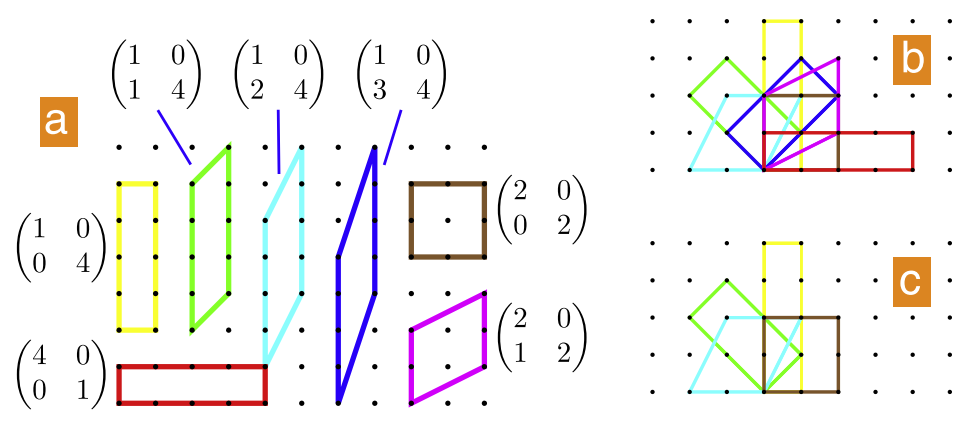
\includegraphics[width=0.86\textwidth]{figs/ch4_2d_square_lattice.png}
  \caption{(a) 7个大小为四倍原晶格的厄米标准型(HNF)基矢量及其对应的单位晶胞。(b)相同的超晶格,但使用最短的(正交的)基向量来描述。(c)这七个晶格去重后的四个完全不等价的超晶格。}
  \label{fig:ch4_2d_square_lattice}
\end{figure}

第二步对于特定的超胞,格点位置可以放置不同的种类的原子构成不同的构型,要判断两个构型之间是否相同,可以通过对一个构型施加其构型对应的所有操作后,再对比另外一个构型以检查这两个构型是否等价。在实际操作中,对结构直接作用对称操作得到新的空间坐标的计算效率并不高,因为针对的是确定格点的结构,格点间的距离是一个多余的参量,不影响等价性的结果,因此可以对特定超胞的不同晶格进行编号,则超胞的商群中的每一个对称操作都会等价于一个置换操作。以二元合金为例,每个构型都可以由一个二进制0,1编号表示,因此可变换对应于一个十进制整数,每一个对称操作所产生的效果仅仅是将一个整数变为另一个整数,我们通过哈希表来储存所有无法通过对称性变换到集合中其他对象的所有非等价的对象。

下面小节详细描述这两步所涉及的细节内容。

\section{晶胞的查重}
晶胞查重的第一步是给出所提供的原始晶格的所有平移不等价超晶格(可包含因旋转操作而重复的晶格),即产生所有的衍生晶胞的初始非平移等价的集合。我们考虑$B=A\cdot H$,这样的晶胞变换,其中$A$是原始晶胞的基矢(为表述清晰,论本表述中使用列向量的形式,但在程序中有时会使用基矢矩阵转置后变为行向量,来表示晶胞的基矢),$H$为作用在原始矩阵的变换矩阵,其元素为整数,$B$则为变换后的基矢。如果$H$是一个行列式为\num{+-1}的矩阵,则变换后的晶胞与原晶胞物理等价,$A$和$B$仅仅是同一套晶胞对应的不同的基矢选择。换言之,如果整数$H$矩阵的行列式为\num{2},则晶格$B$是晶格$A$的超晶格,且为单胞体积其原晶格单胞体积的两倍。

我们设有两个整数矩阵$H_1$,$H_2$,它们有相同的行列式值,如果$H_1$能够通过整数的列操作(列之间的线性运算)变为$H_2$,则他们产生的是同一套晶格。我们将这些操作矩阵的正则形式表示为下三角矩阵的厄米标准型形式,这样能够保证每个超晶格都有且仅有一个矩阵对应(下三角厄米标准型的唯一性\cite{santoro1973coincidence})。三维情况下,下三角矩阵厄米标准型为:

\begin{equation}\label{eq:hnf}
  \begin{pmatrix}
    a & 0 & 0 \\
    b & c & 0 \\
    d & e & f
  \end{pmatrix}, \qquad
  0\leq b < c, \qquad
  0\leq d, e< f.
\end{equation}

这种表示下,矩阵的行列式的值为对角线元素的乘积$a\times c \times f$。同时,该行列式值n也是拓展后超晶格的体积,即将原始晶胞体积看作1时变换后的单胞的体积倍数。在这样的定义下,所有的原始晶格的超晶格对应的变换矩阵$H$,都能够通过指定行列式的值后,将行列式分解为三个整数的乘积形式,再通过式(\ref{eq:hnf})来限制$b$,$d$,$e$的值,从而构造能将原始晶格变换为超晶格的唯一平移不等价的变换矩阵$H$。

综上,给定$H$矩阵的行列式值后枚举所有的H矩阵的算法非常简单,共包含两步:首先,找到$H$行列式的其中一个因数$a$,并保证$1\leq a \leq |H|$,以及第二个对角线因数$c$满足$1\leq c\leq |H|/a$,以及$f$满足$1\leq f\leq |H|/(ac)$。我们以行列式为\num{6}的变换矩阵为例,共可以得到如下表中的所有对角线元素$a$,$c$,$f$的组合。

\begin{table}
  \centering
  \begin{tabular}{c|ccccccccc}
    a & 1 & 1 & 1 & 1 & 2 & 2 & 3 & 3 & 6 \\
    \hline
    c & 1 & 2 & 3 & 6 & 1 & 3 & 1 & 2 & 1 \\
    \hline
    f & 6 & 3 & 2 & 1 & 3 & 1 & 2 & 1 & 1 \\
  \end{tabular}
\end{table}

这一步在程序中可以通过简单的二重循环来实现,分别给出$a$,$c$,$f$的值。在确定对角线元素后我们需要再确定满足条件的$b$,$d$,$e$所有可能的组合。同样这一步也能通过嵌套的三个循环来列出符合条件的$b$,$d$,$e$的值的来完成。
通过生成超晶格后统计数量发现,对于行列式的值为$n=|H|=1,2,3,4,\cdots$的HNF矩阵,其数量为数列:$1,7,13,35,31,91,\cdots$,该数列满足:
\begin{equation}
  \sum_{d|n} d\sigma(d) = \prod^k_{i=1}\left( {\frac{(p_i^{e_i + 2}-1)(p_i^{e_i + 1}-1)}{(p_i-1)^2(p_i+1)}} \right),
\end{equation}
其中$\sigma$为除数函数求和\cite{erdiis1952distribution},$p_i$和$e_i$为$n$的因数和幂次,满足$n=p_1^{e_1}\cdot p_2^{e_2}\cdots p_k^{e_k}\cdot$。

有了明确的数列表达式我们可以验证算法的准确性。同时还需要强调的是,该HNF矩阵的数量是不依赖于原始晶胞的具体形式的,即对所有晶胞都适用。但是这里列出的矩阵仅仅是平移不等价的,针对特定的原始晶胞,在空间中还存在旋转不变形,我们需要去除旋转变换后物理等价的晶胞。而这需要先验知道晶胞的旋转对称操作的信息。

旋转操作仅仅会改变单胞在空间中的朝向,而不会改变晶胞的形状,所以两个形状不同的晶胞一定是非旋转等价的。为了对比形状,可以对晶胞采取了Niggli变换\cite{kvrivy1976unified,grosse2004numerically}变为Niggli标准形式,从而可以直接对比晶格之间的形状,去除旋转等价的晶胞。另外一种去除平移不变形的方法\cite{hart2008algorithm}是通过对HNF矩阵作用后产生的超晶格作用原晶格所拥有的旋转变换$R$,若所有旋转操作均不能使两个晶格重合,则确定这是两个不等价的晶格。在程序中我们选取了两种方式结合的方法来选取不等价的晶格,即首先通过Niggli变换为形式规范的晶胞(Niggli变换后的晶胞的基矢和基矢夹角有确定的大小排列顺序),如果旋转对称操作数量不多我们则作用全部旋转操作查重,如果对称操作过多而候选结构不多,则使用对比每个结构的晶格参数来查重。效率(时间复杂度)上这个方法并没有很大的优势,但是可以确保最后给出的超晶格(操作中是变换格点位置放置不同原子的构型,否则会都变换到统一的原始的晶胞,因为如果不区分格点的元素,则所有晶格都是相同的)都是统一的Niggli变换后的形式,使得后续的处理(格点排列的查重以及后续计算提交)更加简洁。同时,我们还实现了对二维结构的超晶胞的生成和拓展,本文的研究对象是二维材料,所以正好用到了这个对二维拓展的工具(我们的工具软件的链接\cite{pniggli})。

\section{晶体结构的查重}
晶胞的不同是合金材料多样性的基础,如果所有晶格点都是同一种原子,则即便是不同的超晶格也是等价的。所以更重要的是,给定超晶格后,在格点放上元素种类不同的原子,产生新的构型。然而,在摆放上不同原子后,两种构型之间还是有可能经有晶体所拥有的空间群的对称操作互相等价。因此,这一步{\textbf{晶体结构查重}}的目的是对于给定晶胞,在晶胞格点位置放置原子后,生成所有互相不物理等价的构型的集合。

假定我们选定了一个HNF矩阵,则就拥有了其对应的超晶格,即一个包含三个矢量的基组以及原有的格子。我们要将$k$种元素放置在格点上构成特定构型,格点标记为$a$,$b$,$c$...。HNF矩阵描述了晶格的体积为$n$即有$n$个格点(为了简化描述,我们仅以原始晶胞中包含一个原子的格子为例比如面心立方和体心立方的原胞格子,而不是六角密堆的格子其原胞中包含两个不等价的位点,但本节所叙述的方法可以容易的拓展到如六角密堆的格子中\cite{hart2009generating}。拓展到一个原始晶胞包含多个原子,仅仅只是表述上更加复杂,在算法上基本上是完全等价的,我们的软件上实现的是对原胞中包含任意个数原子的晶格的拓展),预将k种元素放在$n$个格点上共有$k^n$种不同的放置方法,但其中的许多摆放方法因为晶格的空间对称性,其两两之间是物理等价的,为了方便描述,我们将每种放置方法对应为一种编号。编号的方法不但方便了描述,通过合理的编号,还能带来了算法上的加速。

我们将摆放原子后的晶格称作晶体结构(或晶体构型),晶体结构的查重问题,就是在所有的$k^n$种结构中选取唯一的不与其他构型等价的构型的问题。早前在上世纪90年代,Ferreira等\cite{ferreira1991stability}实现了FWZ算法来完成这以目的,他们算法是简单的对比任意两个构型,通过作用所有的对称操作来确定是否能由其中一种变换为另外一种,从而判断其等价性。该方法实现上非常直观,但因为要两两对比结构,其时间复杂度为$\mathcal{O}(N^2)$。我们在软件中使用了改进的(编程语言所附带的数据结构层面)源自Hart等在文献\cite{hart2008algorithm}中描述的基于群论的方法来去除不等价的构型的算法,从而实现时间复杂度为$\mathcal{O}(N)$的查重操作。其时间复杂度下降的原因归纳来说,就是对所有构型进行晶胞(从原始晶胞变换扩充后,但格点上还没有区分放置的原子)所拥有的对称操作,从而得到每个构型所对应的衍生结构(个数为晶胞的对称操作数量。但实际算法中,并不需要作用全部的对应空间群中的全部操作,后面我们会看到,具有相同商群的晶格可共享一套编号而一次性进行平移对称性的查重),所有的结构和衍生结构都通过对应的编号表示(编号表示影响的是后续查重的单步时间以及数据存放所占用内存的大小)。再将所有构型(编号表示)进行哈希表的储存,从而仅存放构型不同的对象,构成一个集合(数学上集合的概念,即元素之间不重复)。对构型进行编号的主要作用是:
\begin{enumerate}
  \item 所有构型共用一套格子,通过编号可以节约对构型信息的储存。只需要原始晶胞(格子类型)和HNF矩阵(超晶胞)加上编号就能够还原一个特定构型。
  \item 通过编号,一个构型可以将对构型的一个空间群所拥有的对称操作映射为对应的一个对编号的置换操作,这使得对构型的单步变换操作变得更快。
\end{enumerate}

以三维晶体的结构查重为例,我们来描述如何通过对晶胞格点进行编号来进行查重操作。设拥有一个原始晶胞$L$以及通过H矩阵扩充后的超晶格$S$,$S$是$L$的一个子群(这是显然的,因为$S$的所有群元操作都可以作用在$L$上)。以一种对$S$具有周期性的方式标记$L$等价于仅仅标记商群$G=L/S$的元素。需要注意,因为平移周期性,$L$和$S$有许多种标记方法,但其商群$G$是固定的。与晶格的查询相似的是,我们并不对晶体作用所用的平移操作,而是在其所属的群中进行全部群元操作来查重。具体实现中用到了变换矩阵的史密斯标准型(SNF),即HNF矩阵的对角矩阵,其直接提供了超晶格的商群,SNF的作用是对不同的超晶胞(相同体积扩充后,但不同的HNF矩阵对应的晶胞)进行一个初始归类,因为SNF矩阵的数量大大少于HNF矩阵,从而对于有相同SNF矩阵的晶胞,可以采用相同的编号规则的查重,来一次性去除平移对称操作(即编号的轮换操作)所导致的重复,从而大大减少对每个结构所需要的对称操作数量,因此能够大大降低整体的运行时间。这是因为,SNF矩阵的作用是和编号息息相关的,对于对应相同SNF矩阵的不同HNF矩阵的超晶格,可以共用一套编号方式以及该编号下晶体对称操作映射的对编号的置换操作。

之后,在对一套格子编号后,我们需要对编号进行等价性的判断,仅保留对应唯一不重复构型的编号。其中需要排除的是:
\begin{enumerate}
  \item 编号的轮换对称操作后等价的构型(因为编号本身不影响构型),其实该操作就是前面同类SNF矩阵对应晶胞的平移操作后的等价查重
  \item 编号的交换对称(编号本身不影响构型)
  \item 编号后可缩减为更小的超胞(该条件仅用于已经在较小体积的超晶格中已经统计了这个构型)
  \item 由于晶格旋转对称操作导致的编号置换。
\end{enumerate}
其中前两种属于相同情况,我们在编号的生成时就仅仅生成唯一的序列。针对第三种情况,若一个编号对应的构型能够被缩减为一个更小的构型,那么该编号在其自身的某一个置换操作下一定会等价于其自己,通过这个条件我们可以排除这类构型。实际软件的实现中,我们将这一选项设置为可选,以便用户有时候要仅仅对某一个超晶格来生成所有不等价的构型。而第四种由于旋转对应的置换操作所等价的编号的等价去除方式与之前的晶格判断类似,即作用所有的旋转操作对应的置换操作来实现。

\begin{table}[htb!]
  \centering
  \begin{tabular}{cccc}
    \hline\hline
    n(胞体积) & 二元 & 三元 & 四元 \\
    \hline
    2 & 2      &         &            \\
    3 & 3      &     3    &            \\
    4 & 12      &    13     &    7        \\
    5 & 14      &    23     &    9        \\
    6 & 50      &     130    &    110        \\
    7 & 52      &      197   &      211      \\
    8 & 229      &     1267    &      2110      \\
    9 & 252      &     2322    &       5471     \\
    10 & 685      &    9332     &      32362      \\
    \hline\hline
  \end{tabular}
  \caption{面心立方晶格二元、三元和四元衍生物结构的数目。相比二元构型,三元和四元构型数随着k数量的增加,衍生结构的数量迅速增加。}
  \label{table:derive_structures_num}
\end{table}

需要提到的是,在对结构编号后,对空间构型的操作会变为对编号的置换操作,在程序实现中,我们使用工具spglib\cite{togo2018texttt}来给出所用的对空间构型(超晶胞下而非原晶胞)的对称操作,再对定制编号给出所用对称操作映射的置换操作,并储存成一张表(数据结构上使用一个二维矩阵,每行为一个置换的序列,行数是对称操作的数量)。

至此我们详细描述了构型查重与生成的详细细节,在本章的最后我们给出面心立方晶格,二元,三元,四元下的构型不等价构型数。从表格\ref{table:derive_structures_num}中可以看到当元素种类增加后,构型的数量快速增加。
